\section{Types of Queries}
\label{sec:qtypes}

%\mnote{NO numbers in examples, just explanation}

%This section will illustrate how to derive a metric describing the quantity of information captured
%by tuples flowing through a query processing system based on the assumptions stated in
%Section~\ref{sec:assumptions}.

This section introduces a categorisation of different query types, which is
based on the shape of their graphs. When each operator has at most one successor, the query
graph resembles a tree, with input sources as leaves and one output stream as root. Such queries
belong to the \emph{fan-in} type: the number of edges in the graph decreases from sources
to output. 
A query containing operators with more than one successor instead belongs to a \emph{fan-out} type. 
In this case, the query graph can be more complex, with the restriction of being acyclic. Fan-out
queries can have multiple input sources as well as multiple result streams. 
The following sections provides more detail on these two types of queries.

\subsection*{Fan-in Queries}
\label{sec:fan-in}

\begin{figure}[b!]
	\centering
	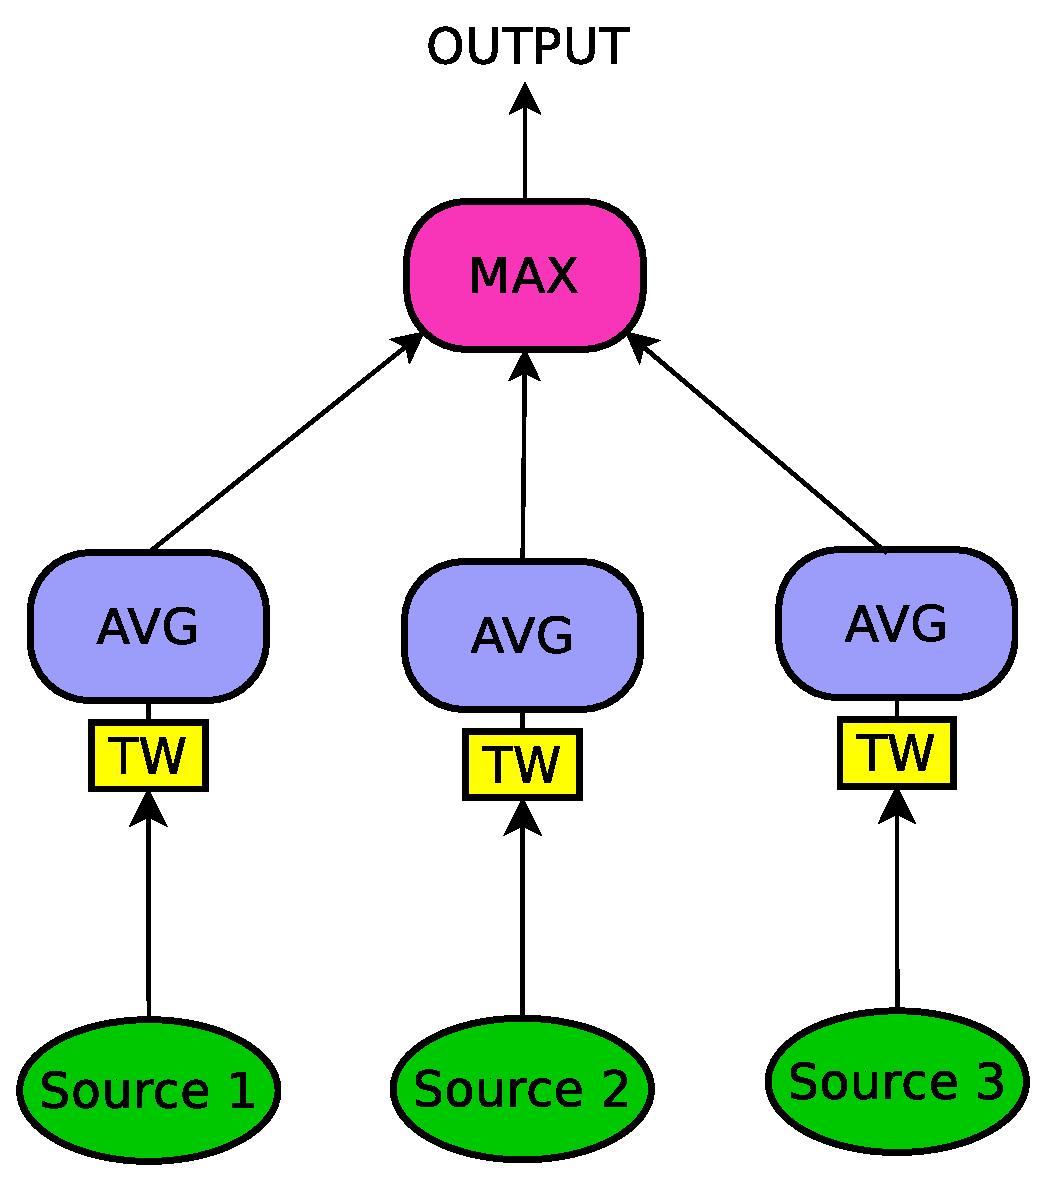
\includegraphics[width=0.35\textwidth]{img/tesi/query_fanin_senza} 
	\caption{An example of a fan-in query. Input values from each source are first averaged over a certain
	time window, and then the maximum is selected.}
	\label{fig:query_fanin}
\end{figure}


In \emph{fan-in} queries, operators have \textit{at most} one successor operator, and the input data from
one or more sources is used to produce a \textit{single result}.
In this category, we find queries computing a single aggregation result.
Such queries have a graph that resembles a tree with many input sources, a series of
processing steps and a single output stream.

\ex Consider the query depicted in Figure~\ref{fig:query_fanin} that calculates
the maximum average value produced by the data sources.
Three sources produce input tuples at different rates. All tuples from a source are first
collected by a time window and then averaged. Finally, the maximum value among the
averages is selected and output. This is a typical fan-in query, in which input tuples from several
sources are collected and processed to produce a single output.

\subsection*{Fan-out Queries} 
\label{sec:fan-out}

\begin{figure}[b!]
	\centering
	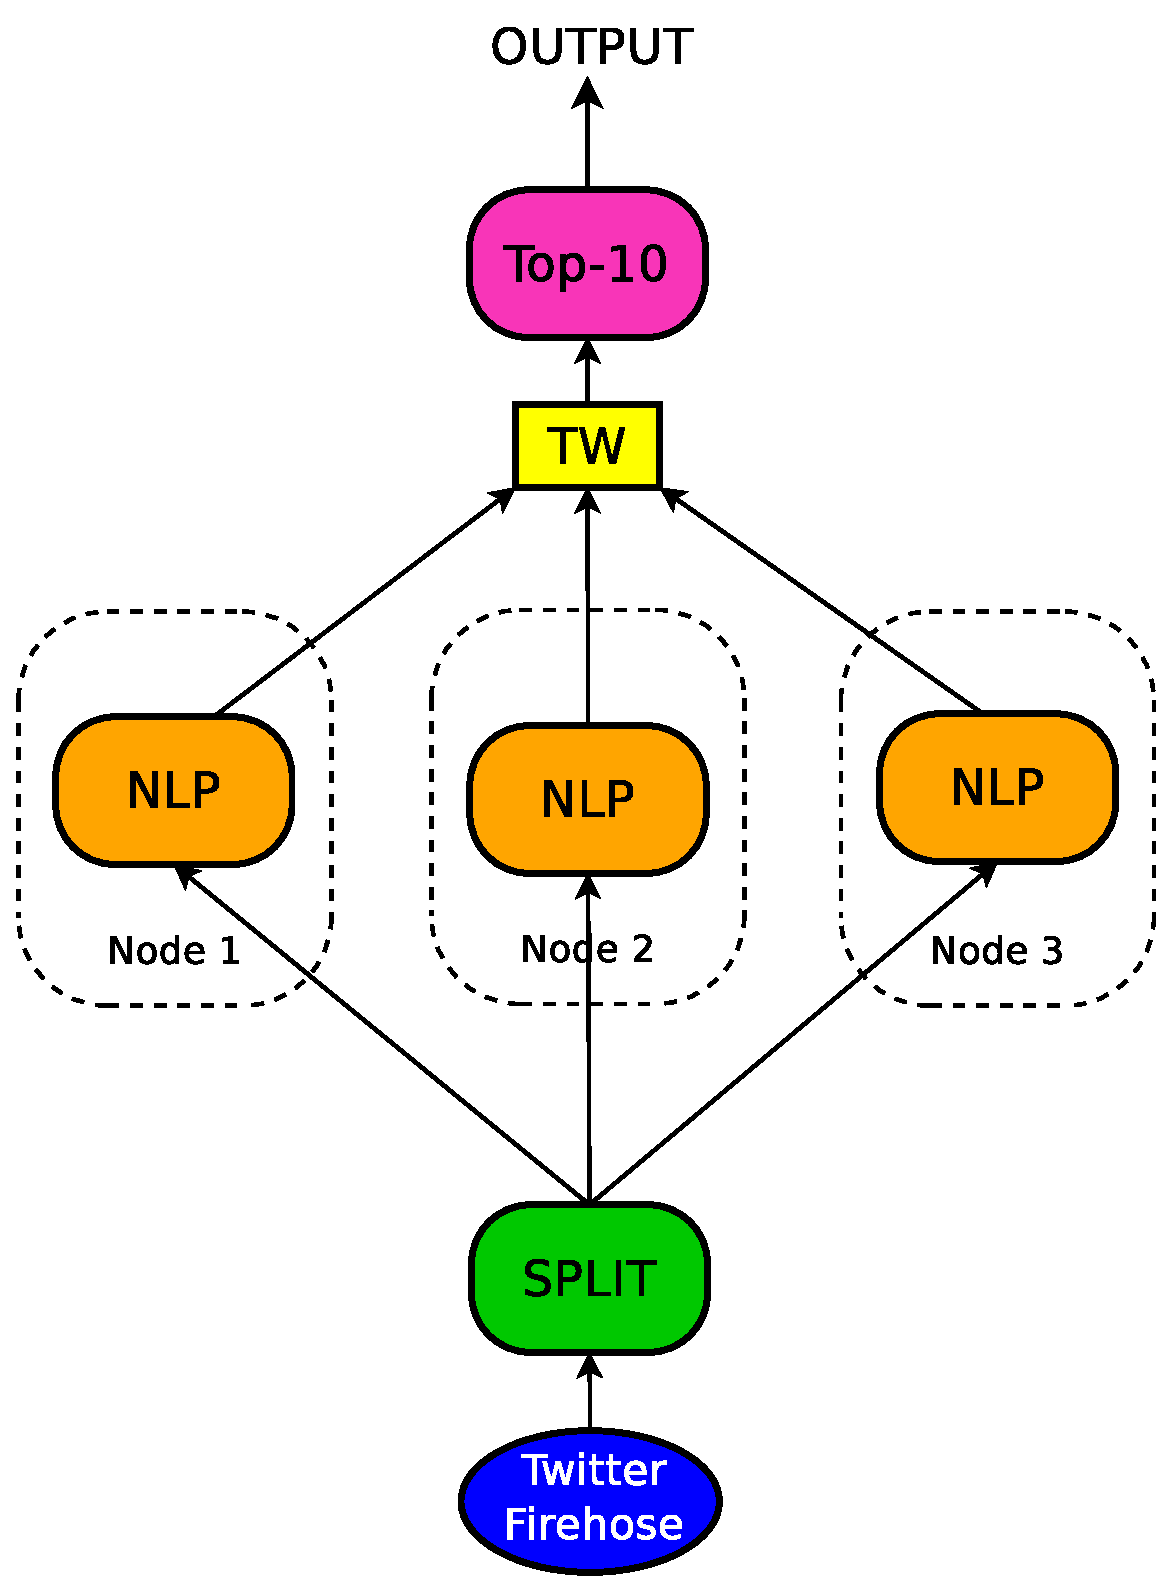
\includegraphics[width=0.45\textwidth]{img/tesi/fan-out_mr_senza} 
	\caption{An example of fan-out query. It processes Twitter data by counting the top-rated messages on a
	certain topic.}
% 	It calculates a value to each tuple based on a natural language processing operator. Due to the heavy
% 	computational cost of these operators, the data is split onto 3 nodes and processed separately. Finally
% 	a max operator determines the message with the highest value.
	\label{fig:fanout_mr}
\end{figure}

The second class of queries that we consider are \textit{fan-out} queries. There one or more operators
send their output to \textit{more than one} downstream operators.
Unlike fan-in queries, whose graph is a tree, a fan-out query
graph can have any configuration, as long as as it does not contain cycles.\\
Fan-out queries can be divided into two possibly overlapping classes: (a) queries with one
result but split computation; and (b) queries with more than one result. Next, we present
examples~for~each~case.

\textbf{Split Computation Queries.} 
Since operators may be computationally too demanding to be hosted on a single processing node, their
computation may have to be split among a number of copies running at different sites. These
copies are composed of the same set of operators but process only a subset of the original data.
Splitting the computation allows the system to spread the processing cost of a set of operators over
multiple nodes and thus overcome an overload condition at a single hosting node. 

\ex Figure~\ref{fig:fanout_mr} shows a query processing Twitter data in
real-time. A stream of Twitter messages can be analysed to calculate the ``top rated'' status updates.
In addition to the message text itself, every message contains information about the location where it
was sent and the author.
\begin{figure}[b!]
	\centering
	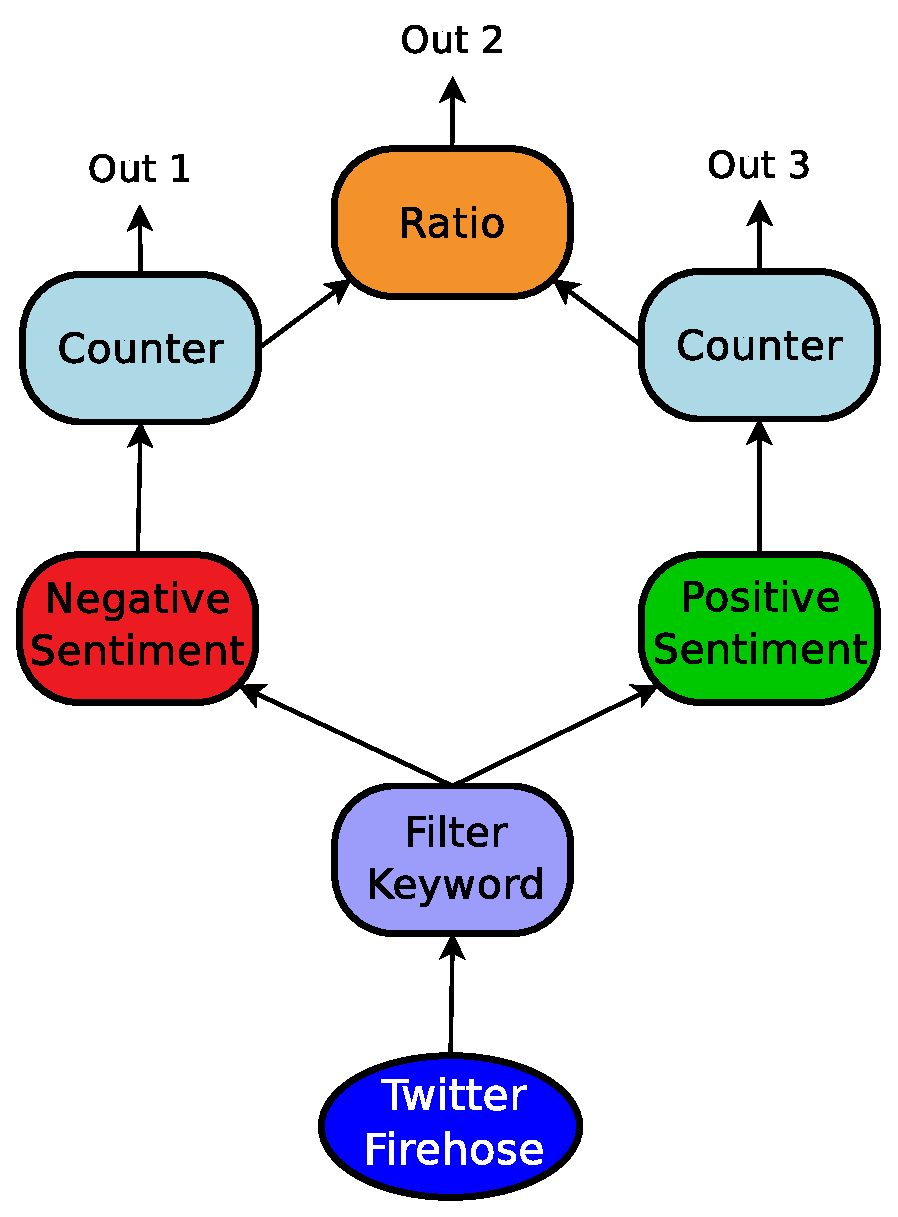
\includegraphics[width=0.4\textwidth]{img/tesi/fan-out_2_senza} 
	\caption{An example of a fan-out query for processing Twitter data. It counts the occurrence of positive
	and negative mentions of a certain keyword and calculates their ratio.}
	\label{fig:query_fanouts}
\end{figure}
A single stream of Twitter messages is split and scattered over three different processing nodes, each
hosting a Natural Language Processing (NLP) operator that calculates some coefficient for each message,
for example, its ``rating''. The output of these NLP operators is collected by a single Top-10
operator preceded by a one minute time-window. The query then outputs then the ten ``top-rated'' Twitter
messages posted every minute. 

\textbf{Multiple Result Queries.} Some queries produce several outputs from the same set of
input data.
These can be seen as multiple single output queries with a partial overlap in their computation. When analysing a
stream of data, a user may be interested in obtaining several different results. Instead of submitting
$N$ queries, they can submit a single fan-out query with multiple end points. Conceptually, this is
simpler than having to design and submit several almost identical queries. It directly exploits the
processing redundancy by reusing a number of streams and operators.


\underline{\textsc{Example}}:~Figure~\ref{fig:query_fanouts} shows a query that calculates the occurrence
of positive and negative statements about particular keywords on Twitter. 
The original stream contains an unsorted stream of messages. First, a filter eliminates all the
messages that do not contain a keyword of interest. After that, the output stream is multiplexed over
two different NLP operators, which forward tweets if they contain
either a positive or a negative mention of a keyword. The resulting streams are sent to a counter
operator, which produces two output streams counting the number of positive and negative references to
a given keyword. The resulting streams from the counter operators are sent to a final operator that
calculates the ratio between them, resulting in an indication of the general feeling about a
keyword. In this query, a single input source is processed to produce~three~different~results.

% The next section will describe the \emph{Source Coverage Ratio} (\sic) quality metric developed in
% the scope of this project, derived following the reasoning of all the model assumptions made in
% Section~\ref{sec:assumptions}.
% In Section~\ref{sec:apps} there will be a further analysis of these sample queries, which will be used as
% running examples of real-world applications of the \sic metric.
 
